%\begin{mdframed}
%    \textbf{La extensión máxima para esta sección es de 4 páginas.} Si utiliza menos páginas y explica bien sus resultados, es preferible.
%\end{mdframed}

%Presente sus resultados mediante \textbf{tablas y gráficos}. Cada tabla o gráfico debe estar referenciado en el texto, con una breve descripción de lo que se observa y por qué es relevante.

%\textbf{Es necesario automatizar la generación de las gráficas}, ya que es imprescindible que se pueda confirmar que las visualizaciones presentadas son producto de los datos generados por sus algoritmos.

%Escoja las gráficas más representativas y que muestren de manera clara los resultados obtenidos. Esta elección es parte de lo que se evaluará en la sección de presentación de resultados.



\subsection{Análisis de resultados: Greedy vs Fuerza Bruta}

\subsubsection{Medición de tiempo de ejecución}

\begin{figure}[H]
    \centering
    % Aquí va la ruta relativa exacta
    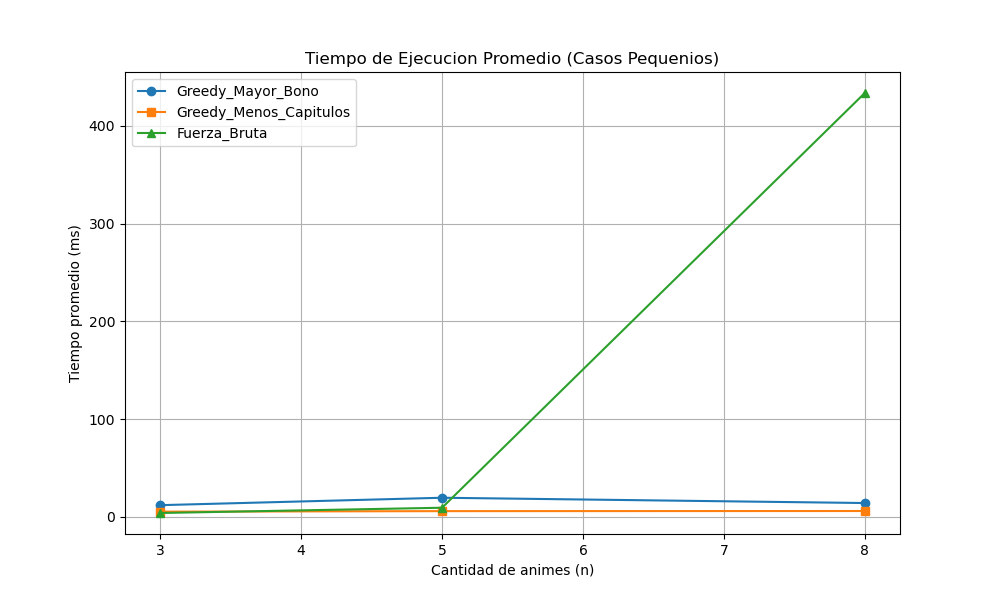
\includegraphics[width=0.8\textwidth]{../code/implementation/data/plots/tiempo_pequenios_plot_promedio.png}
    \caption{Gráfico del tiempo de ejecución promedio para casos pequeños.}
    \label{fig:tiempo_pequenios}
\end{figure}


Este gráfico se centra en visualizar de buena manera la comparación entre el algoritmo de Fuerza Bruta con los algoritmos Greedy. 
La figura deja en evidencia la baja eficiencia del algoritmo de Fuerza Bruta, ya que mientras los Greedy mantienen un tiempo de ejecución pequeño ante tan baja cantidad de animes,
el algoritmo de Fuerza bruta incrementa su tiempo de ejecución de gran manera cuando revisa el caso de 8 animes.


\begin{figure}[H]
    \centering
    % Aquí va la ruta relativa exacta
    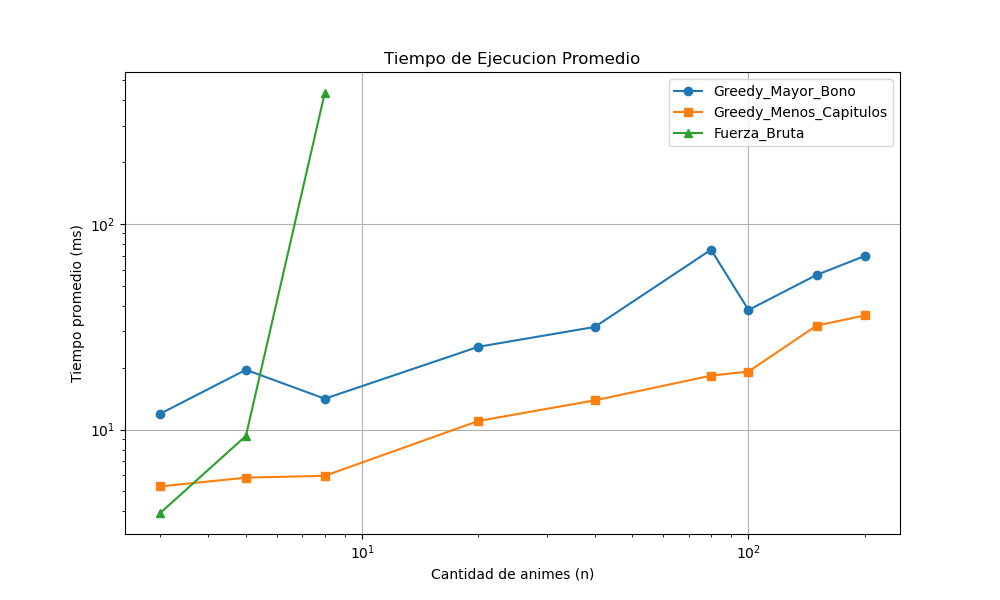
\includegraphics[width=0.8\textwidth]{../code/implementation/data/plots/tiempo_plot_promedio.png}
    \caption{Gráfico del tiempo de ejecución promedio para todos los casos.}
    \label{fig:tiempo_pequenios}
\end{figure}

Puede verse como ambos algoritmos Greedy crecen a ritmo similar mientras que, siguiendo con la idea anterior, se puede notar como al algoritmo de Fuerza Bruta incrementó su tiempo de ejecución de manera exagerada al aumentar la cantidad de animes, dandose la situación de que aún en grandes casos, los algoritmos Greedy tardaban menos que el de Fuerza Bruta con pocos amines.
\\
Tambien podemos notar en este gráfico que inicialmente el algoritmo de Fuerza Bruta es el más rápido de los 3, esto puede deberse a que este algoritmo ya \"directo al punto \", mientras que ambos Greedy comienzan haciendo comparaciones para ver por donde empezar, lo cual en casos muy muy pequeños provoca que tarden más.

\subsubsection{Medición de satisfacción máxima (Calidad de la solución)}

\begin{figure}[H]
    \centering
    % Aquí va la ruta relativa exacta
    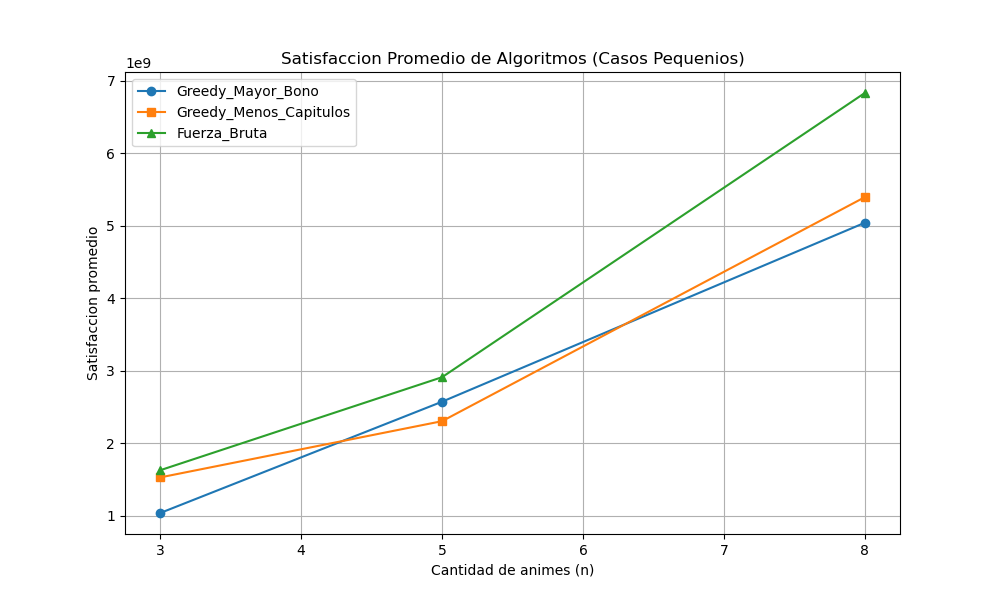
\includegraphics[width=0.8\textwidth]{../code/implementation/data/plots/satisfaccion_pequenios_plot_promedio.png}
    \caption{Gráfico de la satisfacción promedio obtenida para casos pequeños.}
    \label{fig:satisfaccion_pequenios}
\end{figure}

Respecto a la calidad de los resultados, el gráfico muestra lo esperado teóricamente: la Fuerza Bruta siempre alcanza el punto más alto de satisfacción. Al explorar todo el árbol de decisiones, este algoritmo garantiza encontrar la solución óptima absoluta al problema.
\\
Por otro lado, los algoritmos Greedy toman decisiones locales y definitivas sin evaluar el impacto a largo plazo, lo que inherentemente los lleva a soluciones subóptimas y a quedarse por debajo de la cota superior que es Fuerza Bruta. A pesar de esto, se puede observar que logran alcanzar puntajes bastante cercanos al óptimo en una fracción del tiempo. 
\\
Al comparar las dos heurísticas Greedy con el algoritmo de Fuerza Bruta, podemos concluir que los Greedy sacrifican la precisión absoluta a cambio de un tiempo de ejecución viable.




\begin{figure}[H]
    \centering
    % Aquí va la ruta relativa exacta
    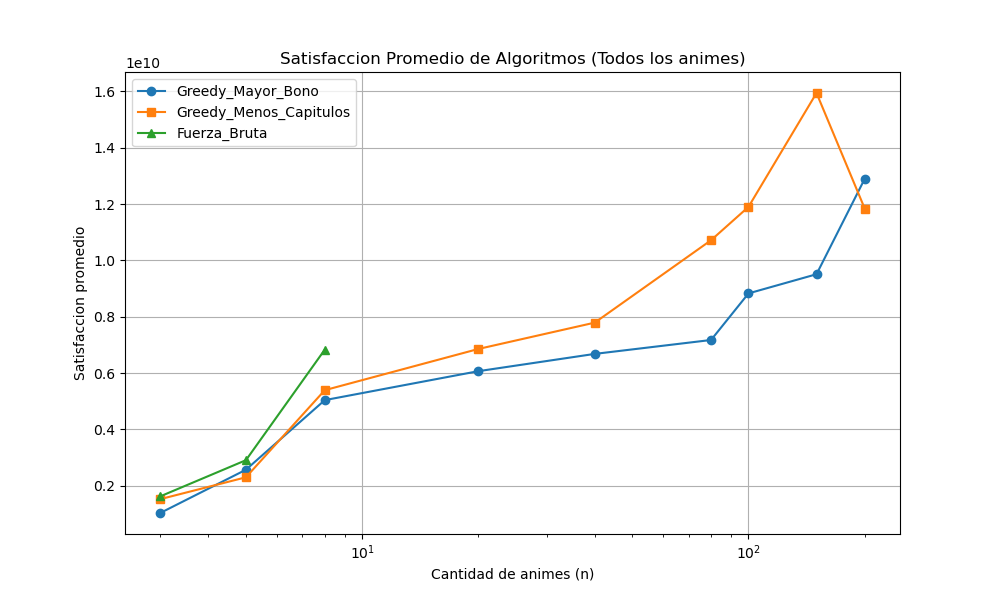
\includegraphics[width=0.8\textwidth]{../code/implementation/data/plots/satisfaccion_plot_promedio.png}
    \caption{Gráfico de la satisfacción promedio obtenida para todos los casos.}
    \label{fig:satisfaccion_pequenios}
\end{figure}

A partir del gráfico podemos deducir que el algoritmo Greedy\_Mayor\_Bono tiende a fallar más que Greedy\_Menos\_Capitulos, ya que este último tiende a obtener mayores valores de satisfacción.



%\begin{mdframed}
%    Recuerde que es imprescindible que se pueda replicar la generación de las gráficas, por lo que usted debe referir a las figuras generadas en `code/implementation/data/plots/`.
%\end{mdframed}
